\chapter{Конструкторский раздел}

В данном разделе будут спроектированы схемы алгоритмов, описаны используемые типы данных, а также произведена оценка памяти и описана структура ПО.

\section{Схемы алгоритмов}

На рисунках 2.1 - 2.2 представлены схемы алгоритмов работы конвейера.

На рисунках 2.3 - 2.5 представлены схемы алгоритмов на конкретных лентах конвейера.

\begin{figure}[H]
	\begin{center}
		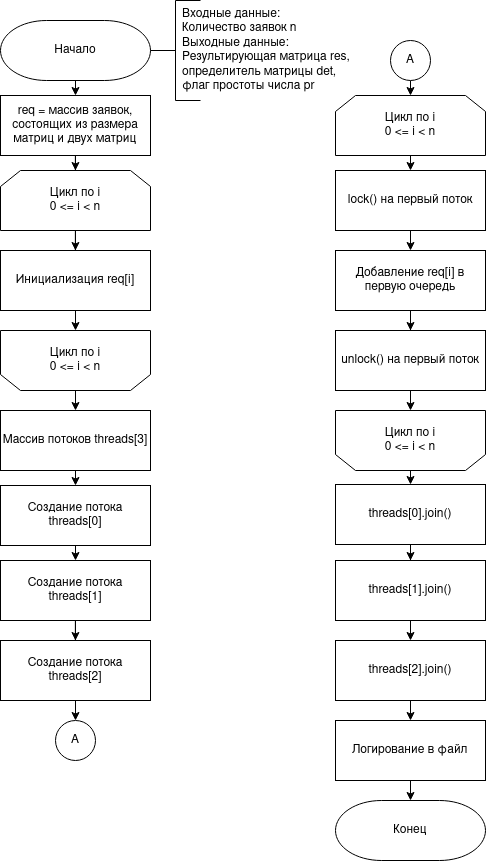
\includegraphics[scale=0.7]{assets/main.png}
	\end{center}
	\caption{Схема главного процесса конвейерной системы}
\end{figure}

\begin{figure}[H]
	\begin{center}
		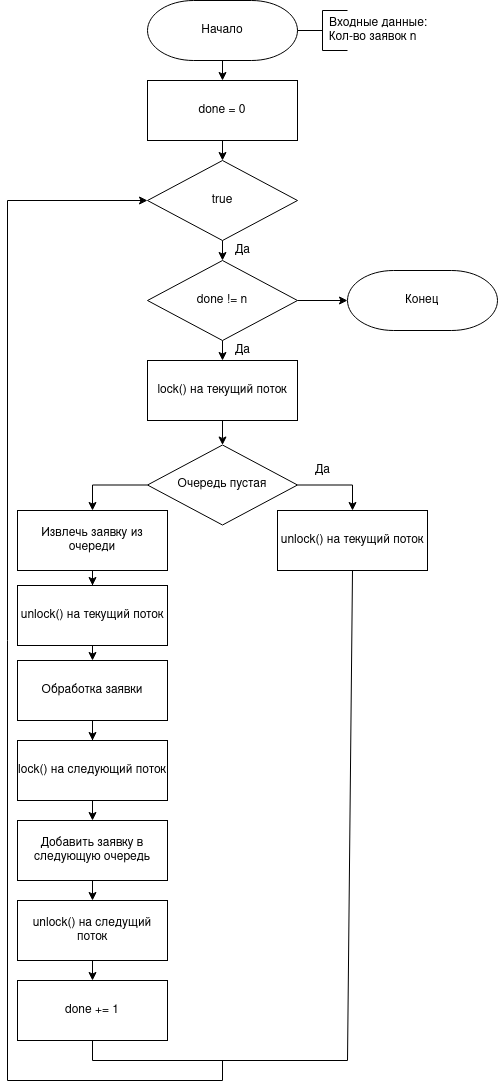
\includegraphics[scale=0.6]{assets/line.png}
	\end{center}
	\caption{Схема работы отдельных лент конвейерной системы}
\end{figure}

\begin{figure}[H]
	\begin{center}
		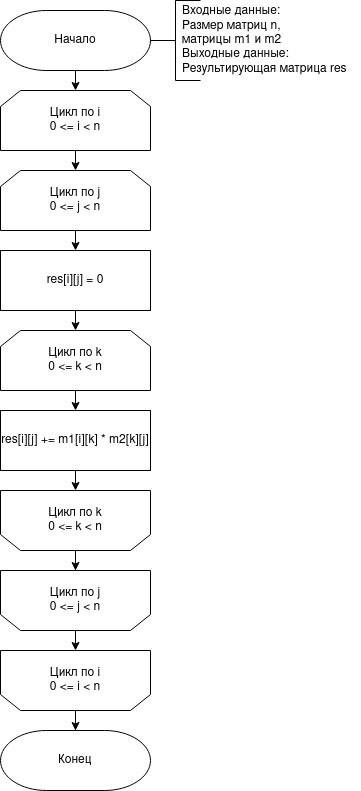
\includegraphics[scale=0.6]{assets/mult.png}
	\end{center}
	\caption{Схема алгоритма умножения матриц (первая лента)}
\end{figure}

\begin{figure}[H]
	\begin{center}
		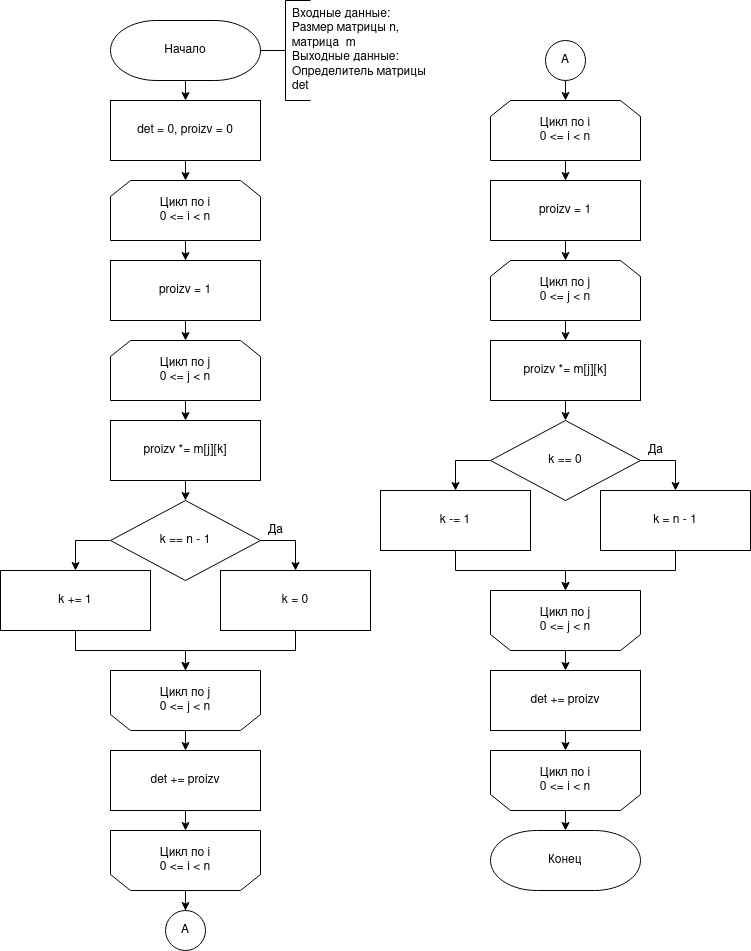
\includegraphics[scale=0.6]{assets/det.png}
	\end{center}
	\caption{Схема алгоритма вычисления определителя матрицы (вторая лента)}
\end{figure}

\begin{figure}[H]
	\begin{center}
		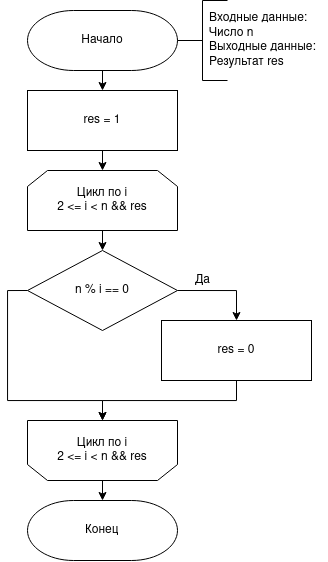
\includegraphics[scale=0.6]{assets/prime.png}
	\end{center}
	\caption{Схема алгоритма определения числа на простоту (третья лента)}
\end{figure}

\newpage
\section{Используемые типы данных}

При реализации алгоритмов будут использованы следующие структуры данных:
\begin{itemize}
	\item потоки - массив типа pthread\_t;
	\item мьютексы - элементы типа pthread\_mutex\_t;
	\item элементы очередей для каждой ленты (листинг 2.1);
	\captionsetup{singlelinecheck = false, justification=raggedright}
	\begin{lstlisting}[caption=Тип данных элементов очереди]
	struct flItem
	{
		int n;
		int **m1;
		int **m2;
		int **res;
		struct flItem *next;
	};
	
	struct slItem
	{
		int n;
		int **m;
		int res;
		struct slItem *next;
	};
	
	struct tlItem
	{
		int n;
		int res;
		struct tlItem *next;
	};
	
	struct reslItem
	{
		int res;
		struct reslItem *next;
	};
	\end{lstlisting}
	\captionsetup{singlelinecheck = false, justification=centering}
	\item общие данные на весь конвейер (листинги 2.2).\newpage
	\captionsetup{singlelinecheck = false, justification=raggedright}
	\begin{lstlisting}[caption=Тип данных для общей информации по конвейеру]
	struct queue
	{
		int num;
		struct flItem *fstart;
		struct flItem *fend;
		struct slItem *sstart;
		struct slItem *send;
		struct tlItem *tstart;
		struct tlItem *tend;
		struct reslItem *resstart;
		struct reslItem *resend;
		pthread_mutex_t m1;
		pthread_mutex_t m2;
		pthread_mutex_t m3;
		pthread_mutex_t resm;
		int startTime;
		int fileMatrix[1000][3][2];
	};
	\end{lstlisting}
	\captionsetup{singlelinecheck = false, justification=centering}
\end{itemize}

\section{Оценка памяти}

Рассмотрим затрачиваемый объем памяти для рассмотренных алгоритмов. 

При последовательном вычислении память используется на:
\begin{itemize}
	\item входные и выходные параметры функций - 3 * n * n * sizeof(int) + 3 * sizeof(int);
	\item вспомогательные переменные - 8 * sizeof(int).
\end{itemize}

В случае конвейерного вычисления память затрачивается также на организацию очереди, а именно:
\begin{itemize}
	\item кол-во заявок в очереди - sizeof(int);
	\item элементы первой очереди - n * sizeof(flItem);
	\item элементы второй очереди - n * sizeof(slItem);
	\item элементы третьей очереди - n * sizoef(tlItem);
	\item элементы результирующей очереди - n * sizeof(reslItem);
	\item мьютексы - 4 * sizoef($pthread\_mutex\_t$);
	\item потоки - 3 * sizeof($pthread\_t$).
\end{itemize}

Таким образом, для конвейерного вычисления затрачивается памяти больше в среднем на n * кол-во заявок в очереди.

\section{Структура ПО}

ПО будет состоять из следующих модулей:
\begin{itemize}
	\item главный модуль - из него будет осуществляться запуск программы и выбор соответствующего режима работы;
	\item модуль интерфейса - в нем будет описана реализация режимов работы программы;
	\item модуль, содержащий реализации алгоритмов.
\end{itemize}

\section{Вывод}

На основе полученных в аналитическом разделе знаний об алгоритмах были спроектированы схемы алгоритмов, выбраны используемые типы данных, проведена оценка затрачиваемого объема памяти, а также описана структура ПО.